\chapter{常见分布}

\section{离散分布}

\subsection{均匀分布}

\begin{definition}[离散均匀分布]
    若随机变量只能在$a_1,\cdots ,a_n$中取值,并且对应的概率相同,则称其遵循\textbf{均匀分布}(Uniform distribution),记为$X \sim U(a_1,\cdots ,a_n)$。
\end{definition}

离散均匀分布的特征:
\begin{description}
    \item[参数] $a_i \in \mathbb{R}$
    \item[概率质量函数] $p(x)=\begin{cases}
                \frac{1}{m} & x=a_1,a_2,\cdots ,a_n \\
                0           & \text{其他}
            \end{cases}$
    \item[矩母函数] $M(t)=\frac{\sum_{i=1}^m e^{a_i t}}{m}$
    \item[均值] $\mu=\frac{\sum_{i=1}^m a_i }{m}=\bar{a}$
    \item[方差] $\sigma^2=\frac{\sum_{i=1}^m (a_i-\bar{a})^2 }{m}$
    \item[实例] 丢一个均匀的骰子
\end{description}

\subsection{Bernouli分布}

\begin{definition}[Bernouli分布]
    若随机变量只能取0或1,并且对应的概率分别为$1-p$与$p$,则称其遵循\textbf{Bernouli分布}(Bernouli distribution)(也称0-1分布),记为$X \sim B(p)$。
\end{definition}

Bernouli分布的特征:
\begin{description}
    \item[参数] $p \in [0,1]$
    \item[概率质量函数] $p(x)=\begin{cases}
                p^x (1-p)^{1-x} & x \in \{0,1 \} \\
                0               & \text{其他}
            \end{cases}$
    \item[矩母函数] $M(t)=p e^t + 1-p$
    \item[均值] $\mu=p$
    \item[方差] $\sigma^2=p(1-p)$
    \item[实例] 丢一次硬币,$p$代表某一面出现的概率
\end{description}

\begin{remark}
    若$A$是一个事件,出现概率为$p_A$,则指示随机变量$I_A$(若$A$出现记为1,否则为0)遵循Bernouli分布,即$I_A \sim B(p_A)$
\end{remark}

\subsection{二项分布}

\begin{definition}[二项分布]
    若进行$n$次独立的Bernouli实验$X_1+\cdots+X_n, X_i \sim B(p)$,则这些随机变量之和$Y=X_1+\cdots+X_n$遵循\textbf{二项分布}(binomial distribution),记为$Y \sim B(n,p)$。
\end{definition}

\begin{figure*}[h]
    \centering
    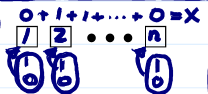
\includegraphics{image/binomail_dist.png}
\end{figure*}

二项分布的特征:
\begin{description}
    \item[参数] $p \in [0,1], n \in \mathbb{N}_+$
    \item[概率质量函数] $p(x)=\begin{cases}
                \binom{n}{x} p^x (1-p)^{n-x} & x \in \mathbb{N}^n \\
                0                            & \text{其他}
            \end{cases}$
    \item[矩母函数] $M(t)=(p e^t + 1-p)^n$,求解方法有:
        \begin{itemize}
            \item \underline{独立变量}之和的矩母函数等于各变量矩母函数之积(参见定理\ref{thm:mgf_sum})
            \item 定义
        \end{itemize}
    \item[均值] $\mu=np$,求解方法有:
        \begin{itemize}
            \item 定义(下述凑一法)
            \item 矩母函数在$t=0$的一阶导
            \item 变量之和的均值等于各变量均值之和
        \end{itemize}
    \item[方差] $\sigma^2=np(1-p)$,求解方法有:
        \begin{itemize}
            \item 定义(下述凑一法)
            \item 矩母函数在$t=0$的二阶导,$\operatorname{Var}(X)=E(X^2)-(E(X))^2$
            \item \underline{独立变量}之和的方差等于各变量均值之和
        \end{itemize}
    \item[实例] 丢$n$次硬币,$p$代表某一面出现的概率,出现此面的次数
\end{description}

\begin{note}
    求解二项分布的均值时,可通过将其凑成概率质量函数之和(为1)的形式:
    \begin{align*}
        E(X) & =\sum_{i=1}^n x \binom{n}{x} p^x (1-p)^{n-x}                 \\
             & = np \sum_{i=1}^n \binom{n-1}{x-1} p^{x-1} (1-p)^{n-1-(x-1)} \\
             & =np
    \end{align*}
    此称为凑一法(sum to one, STO)。同理,求方差时也可使用:
    \begin{align*}
        E(X(X-1))             & =\sum_{i=1}^n x(x-1) \binom{n}{x} p^x (1-p)^{n-x}                   \\
                              & = n(n-1)p^2 \sum_{i=1}^n \binom{n-2}{x-2} p^{x-2} (1-p)^{n-1-(x-1)} \\
                              & =n(n-1)p^2                                                          \\
        \operatorname{Var}(X) & =  E(X(X-1)) + E(X) - (E(X))^2                                      \\
                              & = n(n-1)p^2 + np -n^2 p^2                                           \\
                              & =np(1-p)
    \end{align*}
\end{note}

\begin{proposition}
    二项分布之和仍是二项分布。若$X_1+\cdots+X_k$独立且$X_i \sim B(n_i,p)$,则$Y=X_1+\cdots+X_k  \sim B(n_1+\cdots+n_k,p )$
\end{proposition}

\subsection{几何分布}

\begin{definition}
    若进行无限次独立的Bernouli实验,则第一次出现“1”的实验次数遵循\textbf{几何分布}(geometric distribution),记为$X \sim G(p)$。
\end{definition}

\begin{figure*}[h]
    \centering
    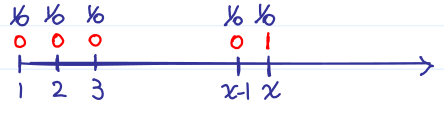
\includegraphics{image/geometric_dist_intu.png}
\end{figure*}

几何分布的特征:
\begin{description}
    \item[参数] $p \in [0,1]$
    \item[概率质量函数] $p(x)=\begin{cases}
                (1-p)^{x-1} p & x \in \mathbb{N}_+ \\
                0             & \text{其他}
            \end{cases}$
    \item[矩母函数] $M(t)=\frac{p e^t}{1-(1-p)e^t}, t<-\ln (1-p)$,求解方法有:
        \begin{itemize}
            \item \underline{独立变量}之和的矩母函数等于各变量矩母函数之积(参见定理\ref{thm:mgf_sum})
            \item 定义
        \end{itemize}
    \item[均值] $\mu=\frac{1}{p}$,求解方法有:
        \begin{itemize}
            \item $E(X)=\sum_{k=1}^{\infty}P(X\ge k)$
            \item 矩母函数在$t=0$的一阶导
            \item 定义(下述微分法)
        \end{itemize}
    \item[方差] $\sigma^2=\frac{1-p}{p^2}$,求解方法有:
        \begin{itemize}
            \item 定义(下述微分法)
            \item 矩母函数在$t=0$的二阶导,$\operatorname{Var}(X)=E(X^2)-(E(X))^2$
        \end{itemize}
    \item[实例] 买彩票时,中奖所需购买张数。
\end{description}

\begin{note}
    微分法求解几何分布均值:
    \begin{align*}
        E(X) & =p\sum_{k=1}^{\infty}k q^{k-1}=p\frac{d}{d q}\sum_{k=1}^{\infty} q^{k} \\
             & =p\frac{d}{d q} \frac{q}{1-q} =\frac{p}{(1-p)^{2}}                     \\
             & =\frac{1}{p}                                                           \\
    \end{align*}
    微分法求解几何分布方差:
    \begin{align*}
        E(X(X-1))             & =p\sum_{k=1}^{\infty}k(k-1) q^{k-1}=p\frac{d}{d q}\sum_{k=1}^{\infty} q^{k} \\
                              & =p\frac{d^2}{d q^2} \frac{q}{1-q} =\frac{2p}{(1-q)^{3}}                     \\
                              & =\frac{2}{p^2}                                                              \\
        \operatorname{Var}(X) & =  E(X(X-1)) + E(X) - (E(X))^2                                              \\
                              & = \frac{2}{p^2} + \frac{1}{p} -\frac{1}{p^2} p^2                            \\
                              & = \frac{1-p}{p^2}
    \end{align*}
\end{note}

\begin{proposition}
    离散分布中有且只有几何分布具备无记忆性:
    \[ P\left\{ X=s+t|X>t \right\} =P\left\{ X=s \right\} \]
\end{proposition}

\begin{proof}
    %TODO 李p135
\end{proof}

\subsection{负二项分布}

\begin{definition}
    若进行无限次独立的Bernouli实验,则第$r$次出现“1”的实验次数遵循\textbf{负二项分布}(negative binomial distribution),记为$X \sim NB(r,p)$。
\end{definition}

\begin{figure*}[h]
    \centering
    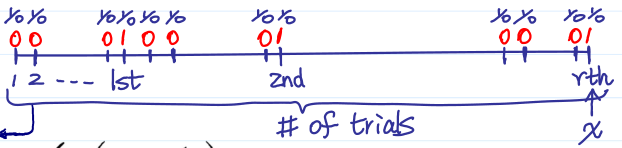
\includegraphics{image/NB_dist_intu.png}
\end{figure*}

负二项分布的特征:
\begin{description}
    \item[参数] $p \in [0,1]$
    \item[概率质量函数] $p(x)=\begin{cases}
                \binom{x-1}{r-1}p^r (1-p)^{x-r} p & x \in \mathbb{N}_r \\
                0                                 & \text{其他}
            \end{cases}$
    \item[矩母函数] $M(t)=\frac{p^r e^{rt}}{(1-(1-p)e^t)^r}, t<-\ln (1-p)$,求解方法有:
        \begin{itemize}
            \item \underline{独立变量}之和的矩母函数等于各变量矩母函数之积(参见定理\ref{thm:mgf_sum,prop:sum_of_geo})
            \item 定义凑一法
            \item 利用公式$\sum_{x=0}^{\infty}\binom{n+x-1}{x}t^x=\frac{1}{(1-t)^n},-1<t<1$
        \end{itemize}
    \item[均值] $\mu=\frac{r}{p}$,求解方法有:
        \begin{itemize}
            \item 定义凑一法
            \item 矩母函数在$t=0$的一阶导
            \item 独立几何分布之和(定理\ref{prop:sum_of_geo})
        \end{itemize}
    \item[方差] $\sigma^2=\frac{r(1-p)}{p^2}$,求解方法有:
        \begin{itemize}
            \item 定义(凑一法)
            \item 矩母函数在$t=0$的二阶导,$\operatorname{Var}(X)=E(X^2)-(E(X))^2$
            \item 独立几何分布之和(定理\ref{prop:sum_of_geo})
        \end{itemize}
    \item[实例] 买彩票时,中奖$r$次所需购买张数。
\end{description}

\begin{proposition}\label{prop:sum_of_geo}
    几何分布之和是负二项分布。若$X_1+\cdots+X_r$独立且$X_i \sim G(p)$,则$Y=X_1+\cdots+X_r  \sim NB(r,p)$
\end{proposition}

\begin{proof}
    %TODO 
\end{proof}

\begin{proposition}
    负二项分布之和仍是负二项分布。若$X_1+\cdots+X_k$独立且$X_i \sim NB(r_i,p)$,则$Y=X_1+\cdots+X_k  \sim B(r_1+\cdots+r_k,p )$
\end{proposition}

\begin{proof}
    %TODO 
\end{proof}

\subsection{多项分布}

\begin{definition}[多项分布]
    若进行$n$次独立的实验,每次实验有$r$种结果,每种结果对于概率分别为$p_1,\cdots ,p_r$。令$X_i$代表得出结果$i$的次数,则随机向量$\mathbf{X}=(X_1,\cdots ,X_r)$遵循\textbf{多项分布}(multinomial distribution),记为$\mathbf{X} \sim Multinomial(n,p_1,\cdots ,p_r)$。
\end{definition}

多项分布的特征:
\begin{description}
    \item[参数] $p_i \in [0,1], \sum_{i=1}^r p_i=1$
    \item[概率质量函数] $p(x)=\begin{cases}
                \binom{n}{x_1 \cdots x_r} p_1^{x_1}\cdots p_r^{x_r} & x \in \mathbb{N}^n \& \sum_{i=1}^r x_i=n \\
                0                                                   & \text{其他}
            \end{cases}$
    \item[矩母函数] $M(t_1,\cdots ,t_r)=(p_1 e^{t_1} +\cdots + p_r e^{t_r})^n$,求解方法有:
        \begin{itemize}
            \item 利用公式
            \item 凑一法
        \end{itemize}
    \item[边缘分布] $X_i \sim B(n,p_i)$
    \item[均值] $E(X_i)=np_i$
    \item[方差] $\operatorname{Var}(X_i)=np_i(1-p_i)$
    \item[协方差] $\operatorname{Cov}(X_i,X_j)=-p_i p_j$,求解方法有:
        \begin{itemize}
            \item 矩母函数求解$E(X_i X_j)$
            \item 凑一法求解$E(X_i X_j)$
        \end{itemize}
    \item[实例]
\end{description}

\begin{remark}
    多项分布是二项分布的泛化。
\end{remark}

\subsection{Poisson分布}

\begin{theorem}[Poisson逼近]\label{thm:Poisson_theorem}
    \[ \lim_{n p_n \to \lambda} \binom{n}{k} p_n^{k} (1-p_n)^{n-k} = \frac{\lambda^{k}}{k !}e^{-\lambda} \]
\end{theorem}

\begin{proof}
    记$np_n=\lambda_n$,记$p_n=\lambda_n/n$,我们可得
    \begin{align*}
        \binom {n}{k} p_n^k(1-p_n)^{n-k} & = \frac{n(n-1)\cdots(n-k+1)}{k!}\left( \frac{\lambda_n}n \right)^k \left( 1 - \frac{\lambda_n}n \right)^{n-k} \\
                                         & = \frac{\lambda_n^k}{k!}\left( 1 - \frac1n \right)\left( 1 - \frac2n \right) \cdots
        \left( 1 - \frac{k-1}n \right)
        \left( 1 - \frac{\lambda_n}n \right)^{n-k}.
    \end{align*}
    对固定的$k$有
    \begin{align*}
         & \lim_{n\to+\infty}\lambda_n = \lambda ;
         & \lim_{n\to+\infty}\left( 1 - \frac{\lambda_n}n \right)^{n-k} = e^{-\lambda} ;
         & \lim_{n\to+\infty}\left( 1 - \frac{1}{n} \right) \cdots \left( 1 - \frac{k-1}n \right) = 1.
    \end{align*}
    从而
    \[
        \lim_{n\to+\infty} \binom{n}{k} p_n^k(1-p_n)^{n-k}  = \frac{\lambda^k}{k!}e^{-\lambda}
    \]
    对任意的$k$($k=0,1,2,\cdots$)成立
\end{proof}

\begin{definition}[Poisson分布]
    若随机变量$X$的概率分布列满足以下形式:
    \[ P(X = k) = \frac{\lambda^k}{k!}e^{-\lambda},\; k = 0,1,2,\cdots, \]
    则称其遵循\textbf{Poisson分布}记为$X\sim P(\lambda)$.
\end{definition}

\begin{remark}
    由定理\ref{thm:Poisson_theorem}可看出,Poisson分布可作为二项分布的近似。$\lambda$的涵义%TODO
\end{remark}

Poisson分布的特征:
\begin{description}
    \item[参数] $\lambda>0$
    \item[概率质量函数] $p(k)=\begin{cases}
                \frac{\lambda^{k}}{k !}e^{-\lambda} & x \in \mathbb{N}^n \\
                0                                   & \text{其他}
            \end{cases}$
    \item[矩母函数] $M(t)=e^{\lambda (e^t -1)}$,求解方法有:
        \begin{itemize}
            \item 利用公式
            \item 凑一法
        \end{itemize}
    \item[均值] $\mu=\lambda$
    \item[方差] $\sigma^2=\lambda$
    \item[实例] 公共汽车站来到的乘客数
\end{description}

\begin{proposition}
    Poisson分布之和仍是Poisson项分布。若$X_1+\cdots+X_k$独立且$X_i \sim P(\lambda_i)$,则$Y=X_1+\cdots+X_k  \sim P(\lambda_1+\cdots+\lambda_k)$
\end{proposition}

\begin{proof}
    %TODO 
\end{proof}

\begin{definition}[泊松过程]
    %TODO 
\end{definition}

\subsection{超几何分布}

\begin{definition}
    设有$N$个产品,其中有$M$个不合格品.若从中不放回地随机抽取$n$个,则其中含有的不合格品的个数$X$服从超几何分布,记为$X\sim h(n,N,M)$.
    \begin{equation}\label{eq2.4.6}
        P(X = k) = \frac{\binom Mk \binom{N-M}{n-k}} {\binom Nn},\; k = 0,1,\cdots,r,
    \end{equation}
    其中
\end{definition}

超几何分布的特征:
\begin{description}
    \item[参数] $r=\min\{M,n\}$,且$M\le N,n\le N,n,N,M$均为正整数.
    \item[概率质量函数] $p(k)=\begin{cases}
                \frac{\binom Mk \binom{N-M}{n-k}} {\binom Nn}  k = 0,1,\cdots,r \\
                0 & \text{其他}
            \end{cases}$
    \item[矩母函数] 存在,但没有简单的表达
    \item[均值] $\mu=\frac{rn}{n+m}$
    \item[方差] $\sigma^2=\frac{rnm(n+m-r)}{(n+m)^2(n+m-1)}$
    \item[实例] 从一个有限总体中进行不放回抽样
\end{description}

\begin{remark}
    若$m,n \to \infty$时有$p_{m,n}=\frac{n}{m+n} \to p$,则超几何分布可近似为二项分布。
    $\frac{\binom {M}{k} \binom{N-M}{n-k}} {\binom {N}{n}}
        \cong \binom{n}{k}p^k(1-p)^{n-k}$
\end{remark}

\section{连续分布}

\subsection{均匀分布}

\subsection{指数分布}

\subsection{Gamma分布}

\subsection{Beta分布}

\section{正态分布及其导出分布}

\subsection{正态分布}

\subsection{卡方分布}

\subsection{t分布}

\subsection{F分布}

\subsection{Cauchy分布}

\section{各分布间关系}

\begin{figure*}[hp]
    \centering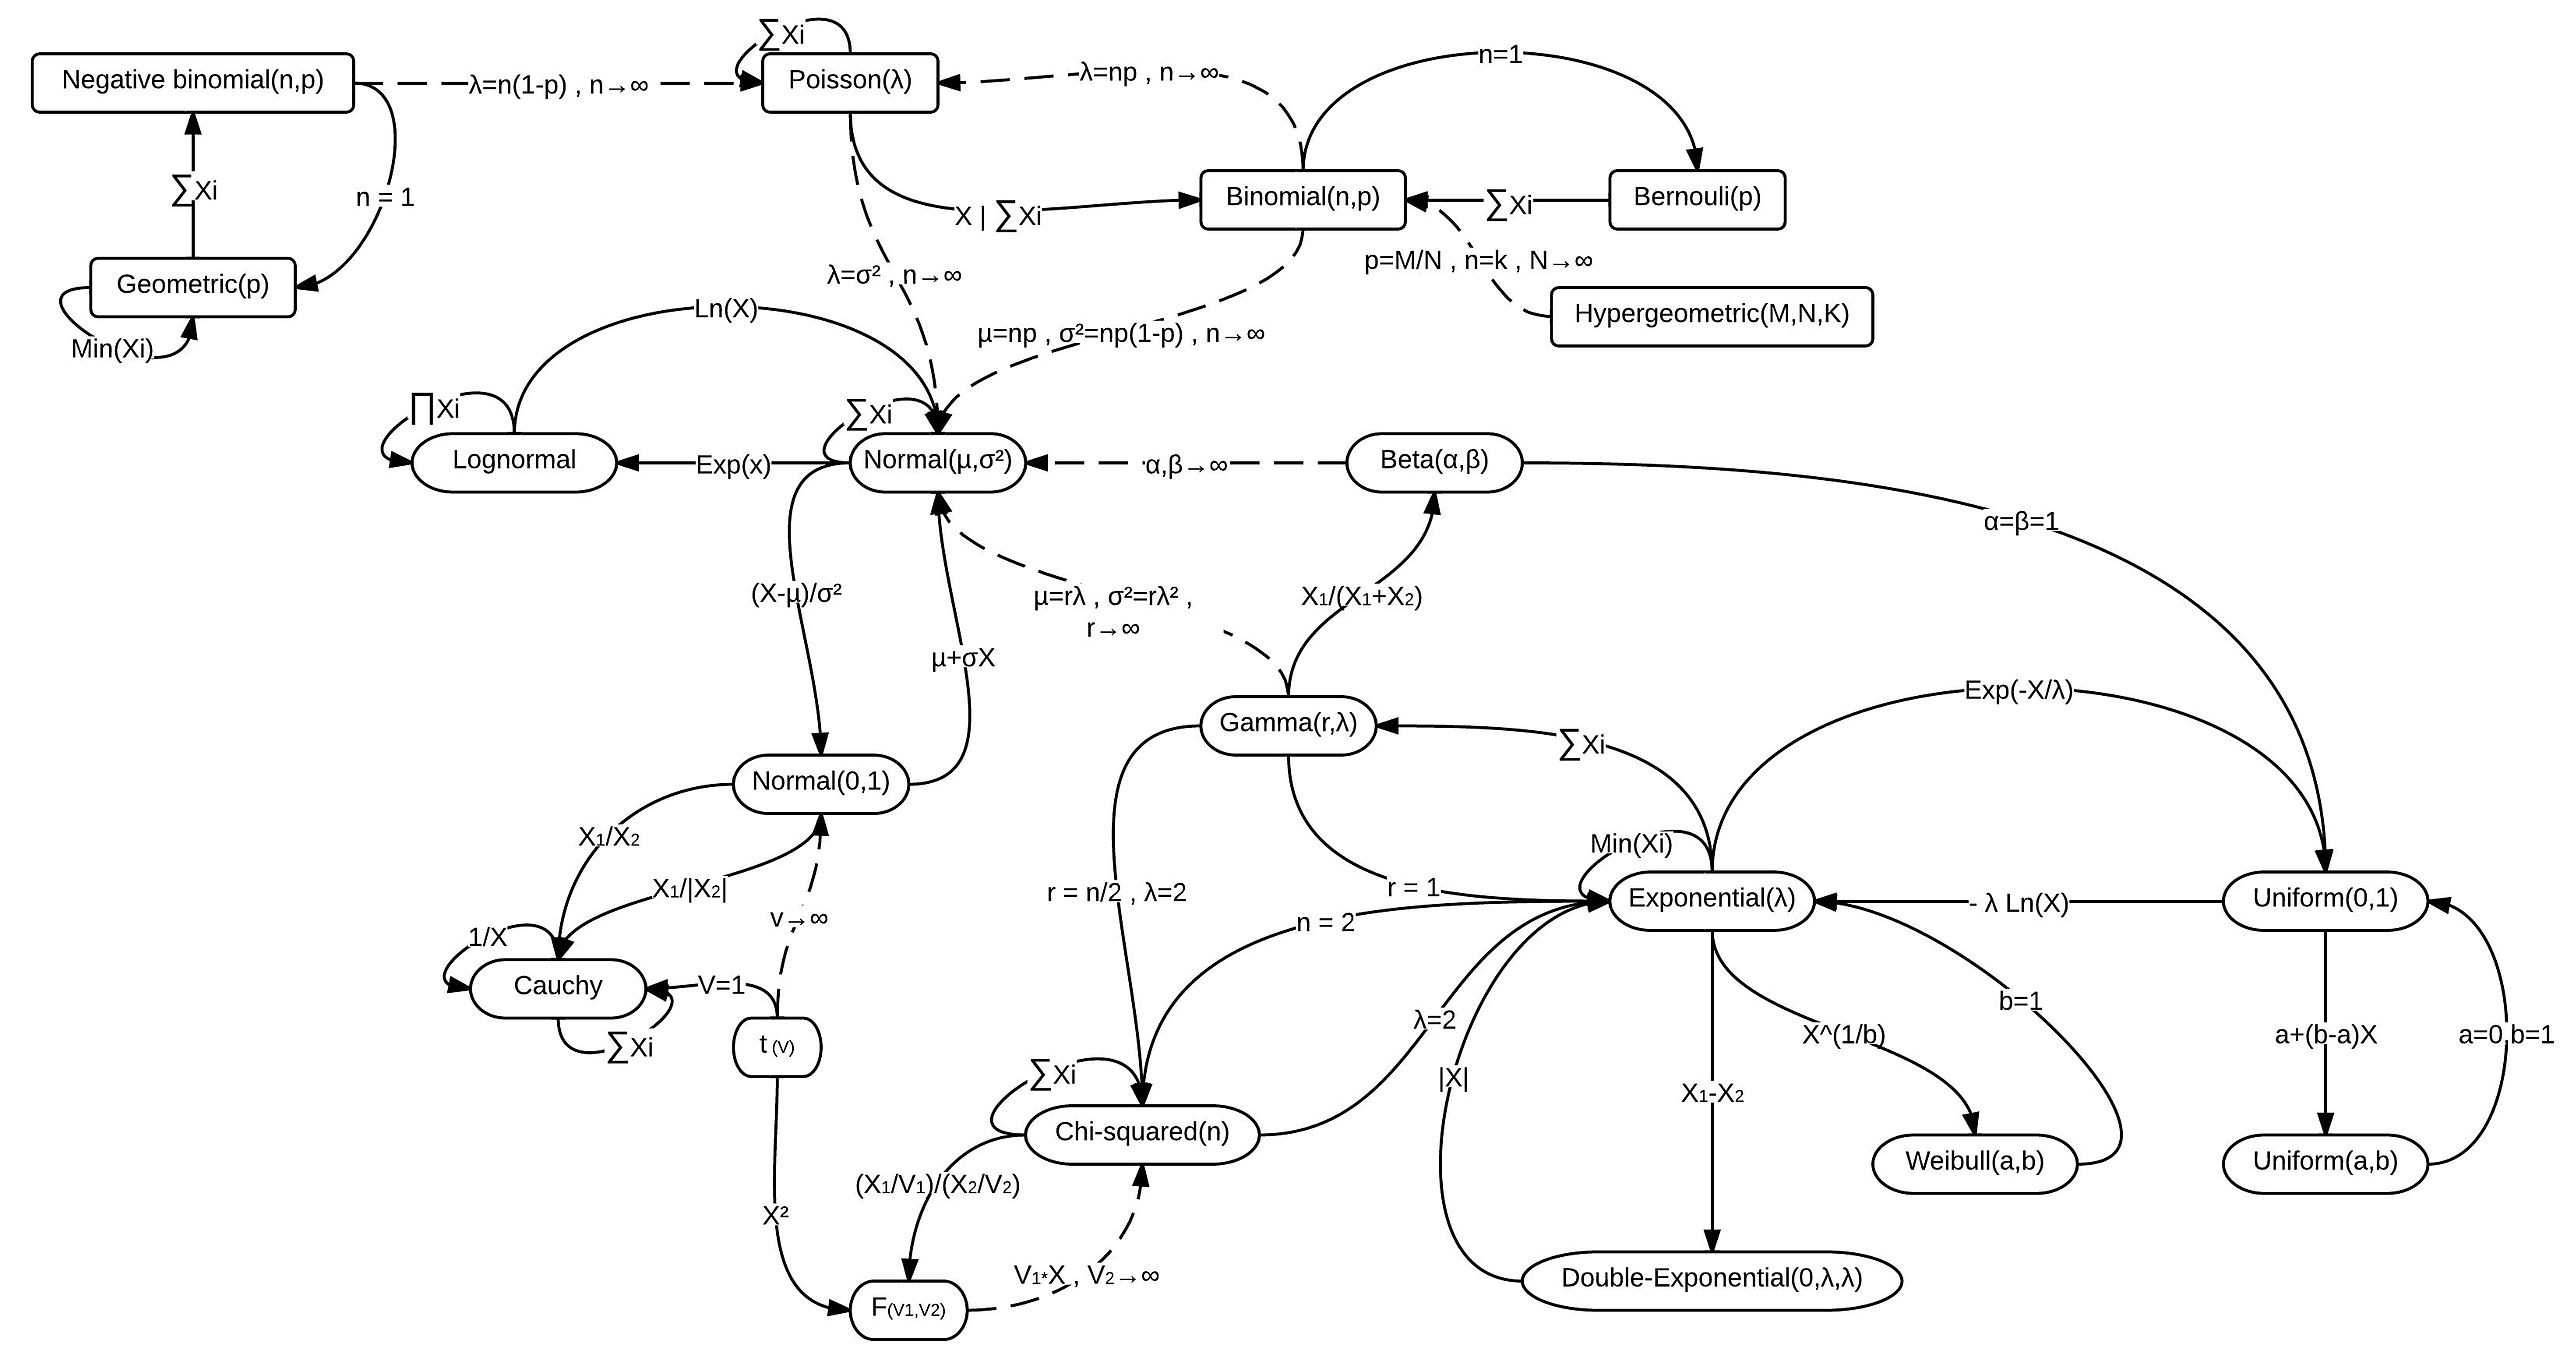
\includegraphics[width=0.95\textwidth]{image/Relationships_among_some_of_univariate_probability_distributions.jpg}
\end{figure*}